% !TEX TS-program = pdflatex
% !TEX encoding = UTF-8 Unicode
\documentclass[a4paper]{article}
\usepackage[english]{babel}
\usepackage[T1]{fontenc}
\usepackage[utf8]{inputenc}
\usepackage{mathtools}
\usepackage[pdftex]{graphicx}
\usepackage{float}
\usepackage{fancyhdr}
\usepackage{geometry}
\usepackage{booktabs} % for much better looking tables
\usepackage{array} % for better arrays (eg matrices) in maths
\usepackage{paralist} % very flexible & customisable lists (eg. enumerate/itemize, etc.)
\usepackage{verbatim} % adds environment for commenting out blocks of text & for better verbatim
\usepackage{subfig} % make it possible to include more than one captioned figure/table in a single float

%%% HEADERS & FOOTERS

\author{Jonathan Karlsson - jonka293 - 890201-1991 \and Niclas Olofsson - nicol271 - 900904-5338}
\pagestyle{fancy} % options: empty , plain , fancy
\renewcommand{\headrulewidth}{1pt} % customise the layout...
\fancyhead[LO,LE]{Laboration 2 - TDDC78}
\lfoot{}\cfoot{\thepage}\rfoot{}
\setlength{\parindent}{0pt}

%%%% SECTION TITLE APPEARANCE

%\usepackage{sectsty}
%\allsectionsfont{\sffamily\mdseries\upshape} % (See the fntguide.pdf for font help)
%% (This matches ConTeXt defaults)
%
%%%% ToC (table of contents) APPEARANCE
%\usepackage[nottoc,notlof,notlot]{tocbibind} % Put the bibliography in the ToC
%\usepackage[titles,subfigure]{tocloft} % Alter the style of the Table of Contents
%\renewcommand{\cftsecfont}{\rmfamily\mdseries\upshape}
%\renewcommand{\cftsecpagefont}{\rmfamily\mdseries\upshape} % No bold!

%%% END Article customizations

%%% The "real" document content comes below...

\title{Laboration 2 - TDDC78}

%\date{} % Activate to display a given date or no date (if empty),
% otherwise the current date is printed

\begin{document}

\maketitle

\section{Program description}
\subsection{Threshold filter}

This program calculates the average intensity of the image and makes all
pixels with a higher-than-average value white, and all other pixels
black.\\

The whole image is read on the main thread. It also calculates the
average intensity of the image. A data structure is created for each new
thread that is to be created. This structure contains the intensity
level, a pointer to the image itself as well as a start and an end value
that defines the area of the image on which the thread is going to apply
the filter. The threads is created and each of them start to work in
their part, since memory is shared the whole image is done when all
threads is done. Each thread is operating on different parts of the
image so there is no risk of memory being overwritten. It is also not
dependent on any other parts of the image, thus making this filter easy
to parallelize.\\

When each thread is done, threads are joined again and the main thread
writes the resulting image to disk.\\

\subsection{Blur filter}

For each pixel this program calculates the average color of the
neighbors with a given radius, of the pixel and sets the pixels color to
the average. This gives a blurred effect over the whole image with a
small radius giving almost the same image back, and a large radius gives a
very blurry image.\\

Just as in the threshold filter, the image is read by the root node.
Gaussian weights needed for the filter is also calculated here. The
structure used for passing parameters to the threds contains some
additional data compared to the thresh filter, such as the generated
Gaussian weights and the blurring radius.\\

Since the resulting value of each pixel depends on neighbour pixel data,
we use different arrays for reading than for writing the resulting
(blurred) image. This way, we do not need any more synchronization since
all write operations is done on different parts of the image. We have
also changed the implementation of the blur filter, so that it only
filters a certain part of the image, depending on the start and end
values calculated by the main thread.\\

After running the filter, threads are joined and the result is written
to disk by the main thread.

\section{Execution times}

In figure \ref{fig:fig1} and figure \ref{fig:fig4} the same number of
nodes is used on different images and we see that the execution time is
increased in a linear manor, for the thresh and blur filter. Figure
\ref{fig:fig2} and figure \ref{fig:fig5} shows how the execution time
decreases with increasing number of nodes for thresh and blur. Figure
\ref{fig:fig3} and figure \ref{fig:fig6} shows how the same increase in
image size and number of nodes give the same execution time, for
\ref{fig:fig6} this is not exactly the case, possibly due to
communication overhead when using too many nodes.

\begin{figure}[h]
  \centering
  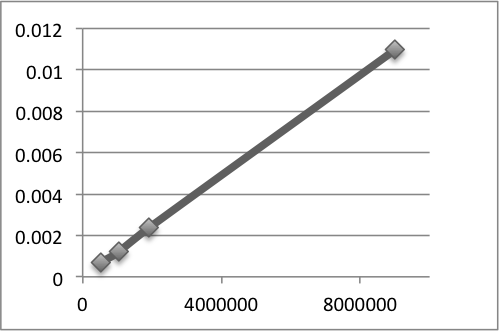
\includegraphics{processor.png}
  \caption{Using the same amount of nodes on different images. (Thresh)}
  \label{fig:fig1}
\end{figure}

\begin{figure}[h]
  \centering
  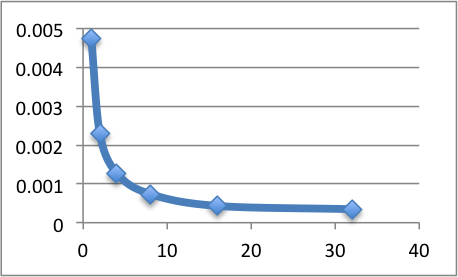
\includegraphics{image.png}
  \caption{Using the same image with different amount of nodes. (Thresh)}
  \label{fig:fig2}
\end{figure}

\begin{figure}[h]
  \centering
  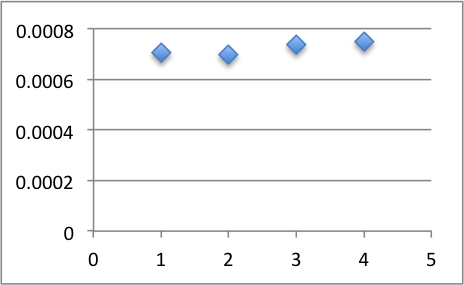
\includegraphics{scale.png}
  \caption{Scaling the image at the same rate as the number of nodes. Using 2, 4, 8 and 38 nodes. (Thresh)}
  \label{fig:fig3}
\end{figure}

\begin{figure}[h]
  \centering
  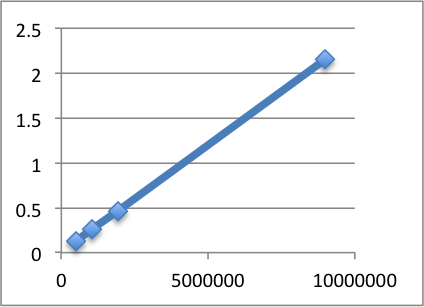
\includegraphics{processorBlur.png}
  \caption{Using the same amount of nodes on different images. (Blur)}
  \label{fig:fig4}
\end{figure}

\begin{figure}[h]
  \centering
  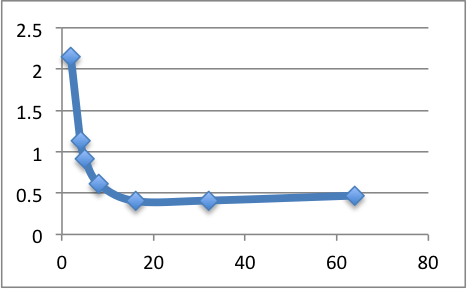
\includegraphics{imageBlur.png}
  \caption{Using the same image with different amount of nodes. (Blur)}
  \label{fig:fig5}
\end{figure}

\begin{figure}[h]
  \centering
  \includegraphics{scaleBlur.png}
  \caption{Scaling the image at the same rate as the number of nodes. Using 2, 4, 8 and 38 nodes. (Blur)}
  \label{fig:fig6}
\end{figure}

\end{document}
